\epigraph{Since the early Middle Ages, mankind has always struggled to increase the hardness and flexibility of metals, to improve the durability and reliability of  metal tools and parts. From the Damascus steel smiths through the swordsmiths of medieval Japan, the method of cold-working metal by the application of precise mechanical pressure such as hammer blows has a glorious history.

In modern times, this concept has reached its apex with industrial surface hardening using shot peening, where thousands of small lead shots are fired at the metal surface, compressing and hardening the surface , improving the durability. With the advent of high power laser systems, an improved process has been developed, the process of laser shock peening.}{\textit{Samuel Zhrdne\\ HoloOr company}}


% because the paragraph alone leaves too much space
\section*{}




Laser shock peening (LSP) is a surface treatment process to improve the fatigue performance of metallic components.
LSP induces residual stresses beneath the treated surface of metallic materials. The residual stresses are produced by a high magnitude shock wave induced by a high-energy laser pulse. The advantage of LSP is that the laser pulse can be adjusted and controlled in real time. A computer-controlled system can measure the energy per pulse and record it for each LSP process on the component \cite{mannava}.

Firstly, this chapter deals with the physical and mechanical mechanisms of laser shock peening. Secondly, it focuses on the parameters of laser shock peening, mainly:

\begin{itemize}
    
    \item laser power density,
    \item pulse shape and duration,
    \item laser wavelength,
    \item laser spot, 
    \item thermal protective coating,
    \item confining overlay,
    \item coverage ratio of impacts.

\end{itemize}

 Lastly, this chapter describes the experimental equipment used for laser shock peening at the HiLASE Centre. 


\section{Laser shock peening overview}

\subsection{Laser shock peening process}
The configuration of an LSP process with a metallic component is shown in Figure \ref{fig:lspconfiguration}. An intense pulsed laser shock beam is focused onto a metal surface for a brief period of time (\SIrange{10}{100}{\ns}). The heated zone is vaporized and transformed to plasma by ionization due to high temperatures (over \SI{10000}{\degreeCelsius} ). The plasma is under high pressure, which propagates through the material via shock waves. Two modes of LSP exist: 

\begin{itemize}

    \item direct ablation mode,
    \item confined ablation mode.

\end{itemize}

The direct ablation mode refers to the interaction of plasma with metal without coating and confinement \cite{sano}. Plasma pressure of tenths of a \SI{}{\GPa} is achieved using direct ablation mode. Higher pressures of \SIrange{1}{5}{\GPa} can be obtained using the confined mode. In the confined mode, the metal surface is usually coated with an opaque material such as black paint or aluminium foil and confined by a material transparent to the laser radiation such as distilled water or borosilicate glass. A stronger pressure pulse results in a higher magnitude of compressive residual stress at a deeper depth \cite{fairland}.

\begin{figure}[h]
    \centering
    
\includegraphics[width=0.6\linewidth]{img/lsp_configuration.jpg}
    \caption{Schematic configuration of laser shock peening process}
    \label{fig:lspconfiguration}
\end{figure}

\subsection{Characteristics of residual stresses induced by laser shock peening}

At high power densities of several \SI{}{\giga\watt\per\cm\squared}, plasma of pressure of several \SI{}{\giga\watt} and a temperature around \SI{10000}{\degreeCelsius} develops on the material surface. The plasma expands rapidly and generates a pressure pulse on the surface of the material. As a consequence, a high-amplitude shock wave propagates through the material. When using the confined ablation mode with a transparent overlay, the plasma is held between the material and the transparent overlay, increasing the plasma's magnitude and amplitude. According to the above-mentioned description of the confined ablation mode, the LSP process can be regarded as a two-step method: 
\begin{enumerate}

    \item uniaxial compression of the irradiated area and dilation of the surface layer is caused by the rapid plasma expansion,
    
    \item the surrounding material reacts to this deformation and generates a compressive stress field.
    
\end{enumerate}

Before the reaction of the surrounding zones excluded from LSP, during the actual LSP process, uniaxial compression is induced in the direction of the shock wave propagation and a tensile state is induced in the plane parallel to the surface. 
After the reaction of the surrounding zones, a compressive stress field is generated in the affected zone, and a tensile stress field is created in the underlying layers. 
The compressive stress field causes deformation in the material. The deformation is plastic as long as the peak dynamic stresses of the shock waves within the material are above the dynamic yield strength of the material. The process of compressive residual stress generation with LSP is shown in Figure \ref{fig:lspresidual}.




\begin{figure}[h]
    \centering
    
\includegraphics[width=0.6\linewidth]{img/residual_stress.jpg}
    \caption{Residual stresses formation with LSP:(a) stretching of impact area during interaction, (b) recovery of material a}
    \label{fig:lspresidual}
\end{figure}

\subsection{Laser shock peening strategy}
During the peening process, a pattern is created made of individual laser pulses. Generally, multiple sequences of the pattern that are gradually shifted across the sample are used to create a layer, as seen in Figure \ref{fig:lspstrategy}. The pattern shifting ensures a more homogeneous residual stress distribution. This strategy's disadvantage is that the protective coating needs to be replaced in between sequences \cite{kaufman}.

\begin{figure}[h]
    \centering
    
\includegraphics[width=0.6\linewidth]{img/lsp_strategy.jpg}
    \caption{Laser shock peening strategy - one layer consisting of four sequences}
    \label{fig:lspstrategy}
\end{figure}

\subsection{Laser system parameters affecting the LSP process}

\subsubsection*{Laser system for laser shock peening overview}

Choosing an appropriate laser system is the first step in fulfilling the LSP process requirements. In LSP laser systems, we are focusing mainly on the following parameters:
\begin{itemize}

    \item pulse energy: \SIrange{1}{100}{\joule}/pulse
    \item pulse duration: less than \SI{100}{\nano\second} 
    
    \item laser wavelength: three wavelengths are used in the LSP process, most commonly:
    
    \begin{itemize}

        \item \SI{1064}{\nano\second} (near-infrared),
        \item \SI{532}{\nano\second} (green),
        \item \SI{355}{\nano\second} (ultraviolet).

    \end{itemize}

\end{itemize}

The laser pulse energy influences the laser power density and therefore the magnitude of surface residual stress. 
The laser pulse duration and temporal shape affect the breakdown threshold of the laser power density. A shorter laser pulse with a short rise time usually results in a higher power density and higher peak pressure. 
The wavelength of the laser system influences the interaction between the laser pulse and the material surface. 

\subsubsection*{Laser spot size and geometry}


\subsubsection*{Laser pulse temporal profile, duration and rise time}


\subsection{Laser shock peening applications}

Nowadays, LSP is heavily commercialized, and hundreds of patents regarding LSP have been issued. The industry leaders are General Electrics, LSP Technologies and Curtis Wright Surface Technologies. LSP is used in the following applications:

\begin{itemize}
 
    \item increase of fatigue life and fatigue strength of structures,
    \item strengthening of thin sections,
    \item hardening surfaces,
    \item shaping or straightening of parts  (laser peen forming),
    \item compacting powdered metals.

\end{itemize}



\section{Laser shock peening station and laser sources at HiLASE Centre}

The HiLASE research centre is an infrastructure focused on laser research and development, located in Dolní Břežany, Czech Republic. HiLASE's Industrial laser applications group (ILA) focuses on LSP, laser induced damage threshold (LIDT), and laser micromachining technologies. ILA is equipped with several experimental stations, including a LSP station. 

The LSP station uses two laser sources:

\begin{itemize}
  \item Bivoj laser system
  \item Litron LPY ST 7875-10 2HG laser 
\end{itemize}

 A laser beam distribution system (LBDS) distributes the beam from the laser laboratory located on the ground floor to the experimental laboratory located on the 1\textsuperscript{st} floor. The Bivoj laser system is a Diode Pumped Solid State Laser (DPSSL) based on Yb-doped gain media with a laser wavelength of 1030 nm capable of delivering energy pulses up to \SI{8}{\joule} at a \SI{10}{\hertz} repetition rate. The beam shape at the output of the Bivoj laser is a square flat-top pulse. An overview of the Bivoj laser system is shown in Figure \ref{fig:bivoj}. The two main sections of the Bivoj laser are the front-end and the \SI{10}{\joule} amplifier.
 
 \begin{figure}[h]
    \centering
    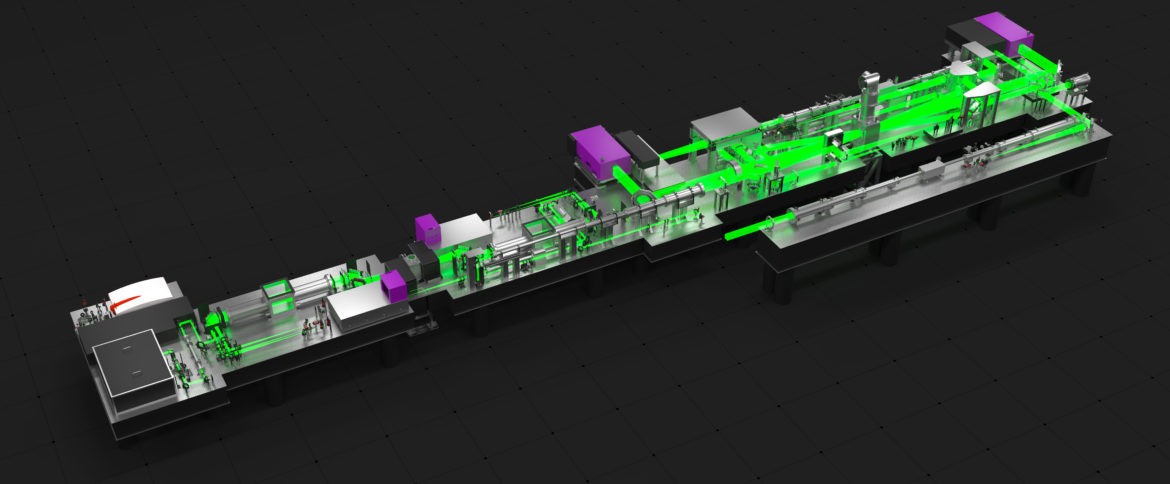
\includegraphics[width=1.0\linewidth]{img/bivoj.jpg}
    \caption{Laser system Bivoj: Diode-pumped solid-state (DPSSL) laser}
    \label{fig:bivoj}
\end{figure}
 
 \subsection{LSP station layout}

The layout of the LSP station is shown in Figure \ref{fig:lsplayout}. The laser beam enters the LSP station through the LBDS output node and
continues to the optical table, where it is redirected and
focused on the target. The target itself is mounted on the
robotic arm. The laser beam position is fixed, so the robotic
arm needs to be moved to direct the laser on the sample.

\begin{figure}[h]
\centering
\begin{subfigure}{.45\textwidth}

    
\includegraphics[width=1\linewidth]{img/lsp_layout.jpg}

    \label{fig:a}
\end{subfigure}
\begin{subfigure}{.45\textwidth}

    \includegraphics[width=1\linewidth]{img/lsp_station_real.JPG}

    \label{fig:b}
\end{subfigure}

\caption{(Description of images from left to right) (1) Schematic layout of LSP station, (2) Photography of LSP station.}
\label{fig:lsplayout}
\end{figure}



\subsection{Bivoj laser system}

\subsubsection*{Bivoj front-end}

The front-end starts with a fibre-based section, consisting
of a fibre oscillator, a fibre amplifier, and a temporal pulse shaper
with \SI{125}{\ps} resolution. The output of the fibre front-end is fed
to the first booster amplifier, which is regenerative and
increases the energy to \SI{30}{\milli\joule} and reduces the repetition rate to \SI{10}{\hertz}. The second booster amplifier works in a multi-pass regime
and increases the pulse energy to approximately \SI{30}{\milli\joule}.
The repetition rate can be switched between \SI{1}{\hertz} and \SI{10}{\hertz}. The
beam shape at the front-end output is \SI{8 x 8}{\mm\squared} square flat top.

\subsubsection*{Bivoj 10 J amplifier}

The \SI{10}{\joule}  amplifier is the first-stage main amplifier based on
cryogenically cooled multislab technology. The principal
component of the amplifier is the amplifier head, where the
gain media are stored and cooled by gaseous helium to 
the temperature of about \SI{150}{\kelvin}. The laser beam from the front-end
is enlarged to \SI{22 x 22}{\mm\squared} and sent to the \SI{10}{\joule} amplifier, where
increases its pulse energy from approximately \SI{30}{\milli\joule} to
approximately \SI{8}{\joule} at \SI{10}{\hertz}. The spatial profile of the laser beam at the output of the Bivoj \SI{10}{\joule} amplifier is shown in Figure \ref{fig:spatialprofile} and the temporal profile is shown in Figure \ref{fig:temporalprofile} \cite{saumyabrata}.

\begin{figure}[h]
    \centering
    
\includegraphics[width=0.6\linewidth]{img/spatial_profile.jpg}
    \caption{Spatial profile of laser beam at output of BiVOJ \SI{10}{\joule} amplifier and approximate dimensions.}
    \label{fig:spatialprofile}
\end{figure}

\begin{figure}[h]
    \centering
    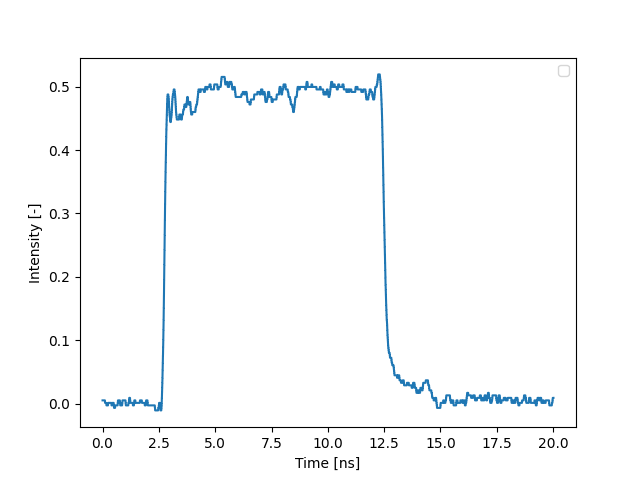
\includegraphics[width=0.6\linewidth]{img/temporal_profile_bivoj.png}
    \caption{Temporal profile of laser beam at output of BiVOJ \SI{10}{\joule}.}
    \label{fig:temporalprofile}
\end{figure}

\subsection{Litron LPY ST 7875-10 2HG laser}

The second laser source available at the LSP station is the Litron LPY ST 7875-10 2HG laser, a tabletop laser located directly in the experimental laboratory next to the LSP station. This laser is a pulsed Q-switched Nd:YAG laser suited for industrial or research applications. The Litron  LPY ST 7875-10 2HG laser comes with a super-gaussian resonator. The most important parameters of this system are highlighted in Table \ref{litronparameters} and the laser system is shown in Figure \ref{fig:litron} \cite{litron}. 


\begin{table}[h!]
\centering
    \begin{threeparttable}
        \begin{tabular}{||c | c||} 
        \hline
            \textbf{Parameter} & \textbf{Value} \\ [0.5ex] 
        \hline\hline
        Repetition Rate [Hz] & 10  \\ 
        \hline
            Output Energy [mJ] & \\
            1064nm & 3500 \\
            532nm & 1750 \\
        \hline
            Beam Diameter [mm] & 15 \tnote{a} \\
        \hline
            Beam Divergence [mrad] & <0.5 \tnote{b} \\ 
        \hline
            Pulse Length @1064nm [ns] & 10-12 \\
        \hline
            Pointing Stability [µrad] & 25 \tnote{c} \\
        \hline
            Timing Jitter [ns] & <0.5 \tnote{d}  \\
        \hline
        \hline
        \end{tabular}
        \begin{tablenotes}
            \small
            \item[a] Peak-to-peak Energy - 99 \% of pulses. 
            \item[b] Full angle for 90 \% of the energy.
            \item[c] Half angle.
            \item[d] Jitter is measured concerning the external Q-switch trigger input.
        \end{tablenotes}
    
        \caption{Litron LPY ST 7875-10 2HG parameters}
        \label{litronparameters}
    \end{threeparttable}
\end{table}

\begin{figure}[h]
    \centering
    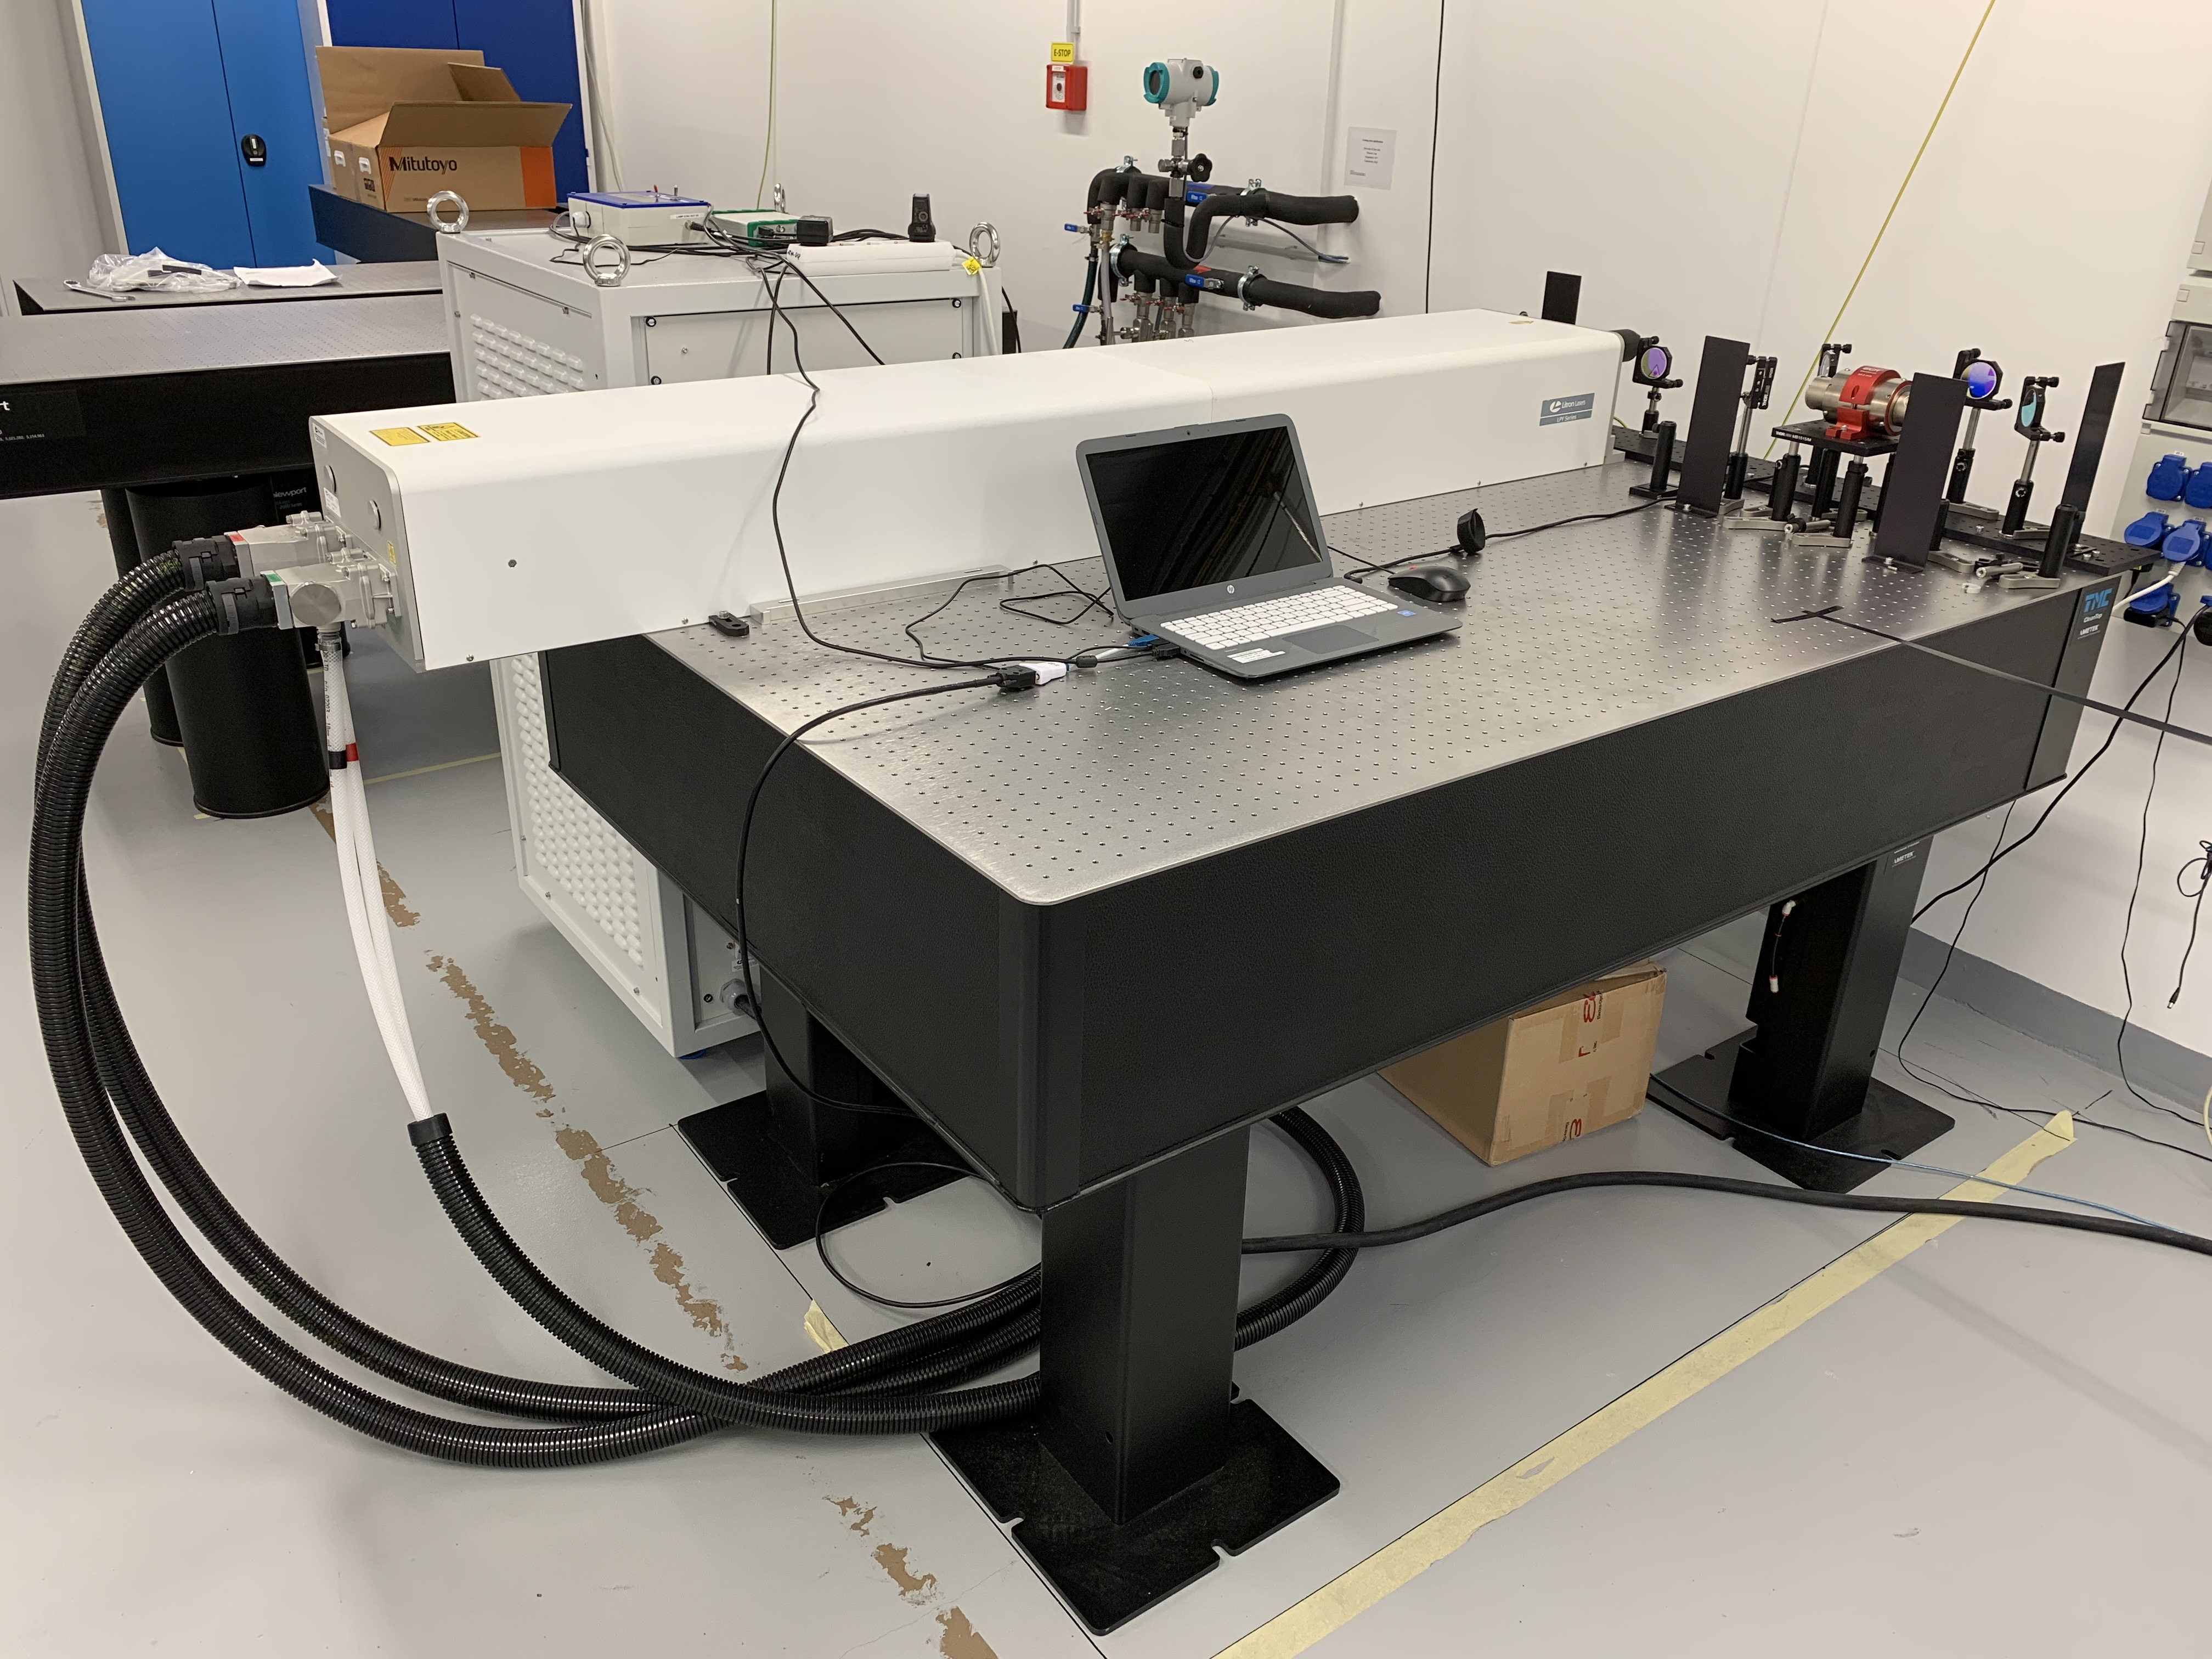
\includegraphics[width=0.6\linewidth]{img/litron.JPG}
    \caption{Litron LPY ST 7875-10 2HG laser at HiLASE Centre.}
    \label{fig:litron}
\end{figure}





\subsection{FANUC M-20iA/20M robotic arm}

The FANUC M-20iA/20M is a 6-axis universal industrial robotic arm with a maximum load capacity at the wrist of \SI{20}{\kg} and a maximum reach of \SI{1811}{\mm}. The repeatability of the robotic arm is \SI{+-0.08}{\mm} The FANUC M-20iA/20M is a multipurpose robotic arm and can be used for various applications such as assembling, packaging and machining.

The robot is coupled with a FANUC R-30iB controller. The R-30iB controller is equipped with a FANUC AIF01A PLC interface module. The interface module is connected to the following expansion modules:

\begin{itemize}
    \item AID16L - 16 digital inputs,
    \item AOD16D - 16 digital outputs,
    \item ADA02A - 2 analog outputs. \cite{fanucunitmanual}
\end{itemize}

The  FANUC M-20iA/20M robot and FANUC R-30iB controller are shown in Figure \ref{fig:robotcontroller} \cite{fanucrobot}.


\begin{figure}[h]
\centering
\begin{subfigure}{.45\textwidth}

    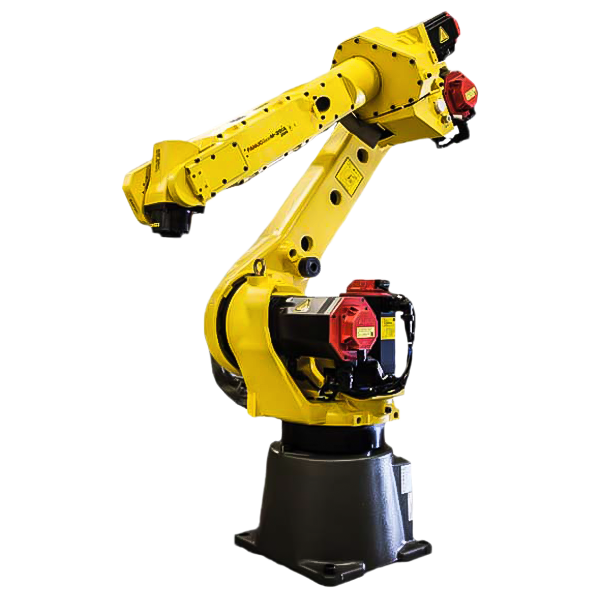
\includegraphics[width=1\linewidth]{img/fanuc_robot.png}

    \label{fig:a}
\end{subfigure}
\begin{subfigure}{.45\textwidth}

    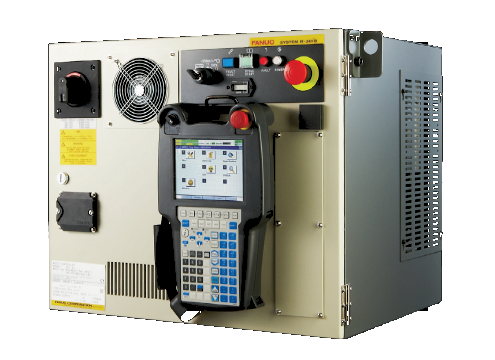
\includegraphics[width=1\linewidth]{img/fanuc_controller.png}

    \label{fig:b}
\end{subfigure}

\caption{(Description of images from left to right) (1) FANUC M-20iA/20M industrial robotic arm, (2) FANUC R-30iB controller with Teach Pendant controller.}
\label{fig:robotcontroller}
\end{figure}



\begin{comment}
\begin{figure}[h]
    \centering
    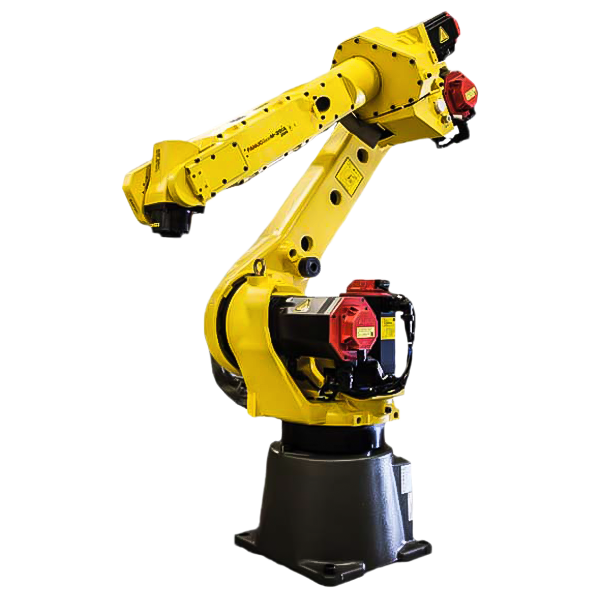
\includegraphics[width=0.6\linewidth]{img/fanuc_robot.png}
    \caption{FANUC M-20iA/20M industrial robotic arm  \cite{fanucrobot}.}
    \label{fig:fanucrobot}
\end{figure}
\end{comment}



\subsection{LSP process example}

The following \href{https://www.youtube.com/watch?v=awhlLU91-dk&ab_channel=HiLASECentre}{video} shows the improvement of cavitation erosion resistance by LSP carried out at the HiLASE centre. This process is developed by HiLASE center and SIGMA GROUP Plc. for the improvement of cavitation erosion resistance of pump blades. The parameters chosen for this experiment are shown in Table \ref{experimentalparameters}. 

\begin{table}[h!]
\centering
    \begin{threeparttable}
        \begin{tabular}{||c | c||} 
        \hline
            \textbf{Parameter} & \textbf{Value} \\ [0.5ex] 
        \hline\hline
        Laser source & Bivoj laser system  \\
        \hline
        Repetition Rate [Hz] & 10  \\ 
        \hline
            Pulse energy at sample [mJ] & \\
            1030nm & 5000 \\
        \hline
            Beam size at sample [\SI{}{\mm\squared}] & 4 \\
        \hline
            Pulse Length @1030nm [ns] & 10 \\
        \hline
            Beam size at sample [\SI{}{\giga\watt\per\cm\squared}] & 5.56 \\

        \hline
        \hline
        \end{tabular}

        \caption{Experimental parameters of Laser Shock Peening for improvement of cavitation erosion resistance.}
        \label{experimentalparameters}
    \end{threeparttable}
\end{table}

